\documentclass{article}
\usepackage[utf8]{inputenc}

% Símbolos
\usepackage{recycle}
\usepackage{amsmath}
\usepackage{amsfonts}
\usepackage{amssymb}
\usepackage{float}
\restylefloat{table}
\usepackage{hyperref}

% Short labels
\usepackage[shortlabels]{enumitem}

% Multicol
\usepackage{multicol}

% Figuras
\usepackage{mathrsfs}
\usepackage{amsmath}
\usepackage{caption}
\usepackage[font=footnotesize]{caption}
\usepackage{graphicx}
\graphicspath{{img/}}
\usepackage{tikz}
\usetikzlibrary{trees}

% Colores
\usepackage{xcolor}
\definecolor{codegreen}{HTML}{9ccb74}
\definecolor{codegray}{rgb}{0.5,0.5,0.5}
\definecolor{codepurple}{HTML}{b48ead}
\definecolor{backcolour}{HTML}{2e3440}

% Márgenes
\usepackage{geometry}
\geometry{showframe=false, headheight=1cm}
\geometry{margin=30mm, bottom=30mm}

% Title size
\usepackage{titlesec}
\titleformat{\section}
{\normalfont\large\bfseries}{\thesection}{1em}{}

% Header & Footer
\usepackage{fancyhdr}
\fancypagestyle{fancy}{
\renewcommand{\footrulewidth}{0.5pt}
\fancyhf{}
\fancyhead[R]{Examen Parcial 3}
\fancyhead[L]{UNAM, Facultad de Ciencias}
\fancyfoot[L]{Inteligencia Artificial 2023-1}
\fancyfoot[R]{\thepage}
}

\fancypagestyle{firstpage}{
\renewcommand{\footrulewidth}{0.5pt}
\renewcommand{\headrulewidth}{0pt}
\fancyhf{}
\fancyfoot[L]{Inteligencia Artificial}
\fancyfoot[R]{\thepage}
}

% Custom Commands
\newcommand{\dollar}{\mbox{\textdollar}}

% Import files
\usepackage{subfiles}

% Title
\title{Tarea 1}
\author{ 
  \small Anzaldúa Díaz Andrea Fernanda \and
  \small Escobar Rosales Luis Mario \and
  \small Garcia Toxqui Demian Oswaldo \and
  \small Padilla Lara Diego Javier
}
\date{\today}

\pagestyle{fancy}

\begin{document}
%%%%%%%%%%%%%%%%%%%% TITLE PAGE %%%%%%%%%%%%%%%%%%%%
  %\begin{titlepage}
  %  %\subfile{sections/title_page}
  %  Insert titlepage here
  %\end{titlepage}
%%%%%%%%%%%%%%%%%%%%%%%%%%%%%%%%%%%%%%%%%%%%%%%%%%%%
\maketitle \thispagestyle{firstpage}

\begin{enumerate}[\textbf{4.}]
  \item \textbf{Búsqueda Informada}
  \begin{itemize}[1.]
    \item Consultando el mapa del sistema ferroviario mexicano 
    \href{https://www.ferromex.com.mx/ferromex-lo-mueve/sistema-ferromex.jsp}{$^{1}$} 
    \href{https://www.gob.mx/cms/uploads/attachment/file/559748/SFM_2020_ESQUEMATICO_.pdf}{$^{2}$} 
    e información proporcionada en la página de \href{https://www.ferromex.com.mx/herramientas/tabla-de-distancias.jsp?eorigen=FXE_09699&edestino=FXE_00929&distancia=1799.9}{Ferromex} (además de unas consultas en Google), 
     tenemos la siguiente tabla de distancias entre estaciones de tren:

    \vspace{3mm}
    \begin{center}
      \begin{tabular}{l l c}
        \textbf{Origen} & \textbf{Destino} & \textbf{Distancia (km)} \\
        \hline 
        Piedras Negras & Monclova & 237 \\ %ojo
        Piedras Negras & Saltillo & 438.11 \\
        Piedras Negras & Monterrey & 437.8 \\
        \hline
        Saltillo & Torreón & 370 \\
        Saltillo & Monterrey & 86.9 \\
        Saltillo & Rio Verde & 437.8 \\
        Saltillo & Querétaro & 639.4 \\
        \hline
        Monclova & Escalón & 535.1 \\
        \hline
        Escalón & Torreón & 181 \\
        \hline
        Torreón & Durango & 252.5 \\
        Torreón & Felipe Pescador & 315.7 \\
        Torreón & Querétaro & 805.4 \\
        \hline
        Durango & Tampico & 905.6 \\
        \hline
        Felipe Pescador & Ciudad de México & 756.9 \\
        \hline
        Ciudad de México & Medias Aguas & 567.3 \\ 
        Ciudad de México & Veracruz & 419.2 \\
        \hline
        Monterrey & Tampico & 515.8 \\
        Monterrey & Río Verde & 554.2 \\
        \hline
        Río Verde & Querétaro & 307.9 \\
        \hline
        Querétaro & Ciudad de México & 218.9 \\
        \hline
        Veracruz & Medias Aguas & 283.8 \\
        \hline
        Medias Aguas & Salina Cruz & 236.2 \\
      \end{tabular}
    \end{center}
  \end{itemize}

  \vspace{3mm}
  A continuación tenemos la tabla de heurística, que generamos usando las distancias 
  por carretera arrojadas por Google Maps:

  \begin{center}
    \begin{tabular}{l l c}
      \textbf{Origen} & \textbf{Destino} & \textbf{Distancia (km)} \\
      \hline 
      Monclova & Salina Cruz & 1644.2 \\[2pt] %ojo
      Saltillo & Salina Cruz & 1566.3 \\[2pt] %ojo
      Monterrey & Salina Cruz & 1445.4 \\[2pt] %ojo
      Escalón & Salina Cruz & 1890.9 \\[2pt] %ojo
      Torreón & Salina Cruz & 1737.4 \\[2pt] %ojo
      Durango & Salina Cruz & 1635.4 \\[2pt] %ojo
      Felipe Pescador & Salina Cruz & 740.2 \\[2pt] %ojo
      Querétaro & Salina Cruz & 939.5 \\[2pt] %ojo
      Tampico & Salina Cruz & 928.1 \\[2pt] %ojo
      Río Verde & Salina Cruz & 897.1 \\[2pt] %ojo
      Ciudad de México & Salina Cruz & 739.9 \\[2pt] %ojo
      Veracruz & Salina Cruz & 503.9 \\[2pt] %ojo
      Medias Aguas & Salina Cruz & 236.2 \\[2pt] %ojo
    \end{tabular}
  \end{center}

  \vspace{3mm}
  Y ya con toda la información recabada se genera el siguiente árbol
  \begin{center}
  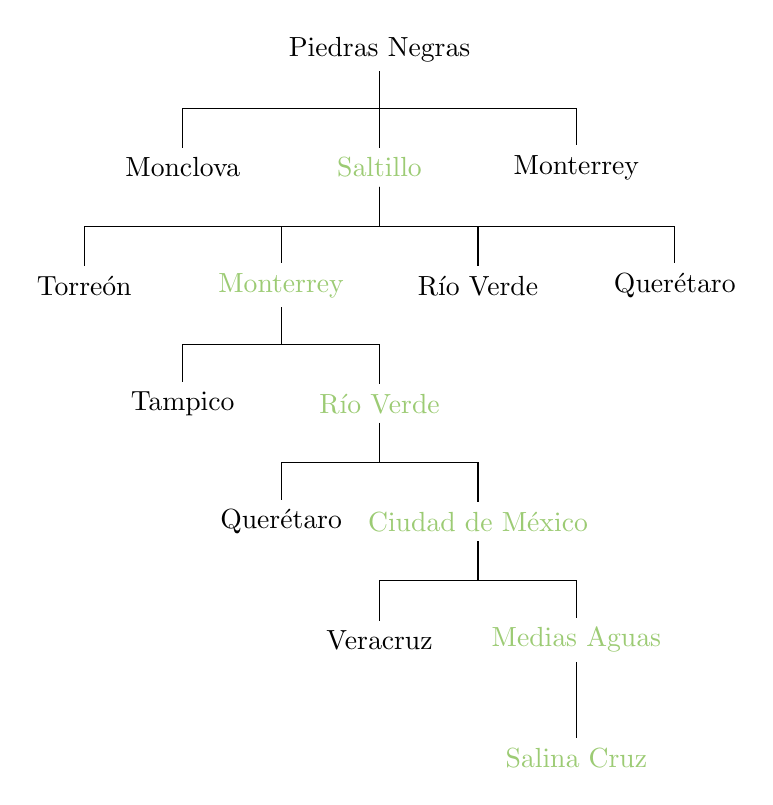
\begin{tikzpicture}
    [
      edge from parent fork down
    ]
    \node {Piedras Negras} [sibling distance = 2.5cm]
        child {node {Monclova}} 
        child {node [codegreen] {Saltillo}
        child {node {Torreón}}
        child {node [codegreen] {Monterrey}
          child {node {Tampico}}
          child {node [codegreen] {Río Verde}
            child {node {Querétaro}}
            child {node [codegreen] {Ciudad de México}
              child {node {Veracruz}}
              child {node [codegreen] {Medias Aguas}
                child {node [codegreen] {Salina Cruz}}
              }
            }
          }
        }
        child {node {Río Verde}}
        child {node {Querétaro}}
        }
        child {node {Monterrey}};
  \end{tikzpicture}
  \end{center}

\end{enumerate}

\end{document}